\documentclass[15pt,a4paper]{article}

%use the english line for english reports
%usepackage[english]{babel}
\usepackage[portuguese]{babel}
\usepackage[utf8]{inputenc}
\usepackage{indentfirst}
\usepackage{graphicx}
\usepackage{moreverb}
\usepackage{subfig}
\usepackage{float}
\usepackage{url}
\usepackage{color}
\usepackage{listings}



\floatstyle{ruled}
\newfloat{code}{!ht}{lop}
\floatname{code}{Código fonte}


\begin{document}

\setlength{\textwidth}{16cm}
\setlength{\textheight}{22cm}


%************************************************************************************************
%************************************************************************************************

\title{
	\Huge\textbf{Breakthrough}
	\linebreak\linebreak\linebreak
	\Large\textbf{Relatório}
	\linebreak\linebreak
	
\includegraphics[height=6cm, width=7cm]{feup.pdf}
	\linebreak \linebreak
	\Large{Mestrado Integrado em Engenharia Informática e Computação}
	\linebreak\linebreak
	\Large{Programação em Lógica}\linebreak
}


\author{\textbf{Grupo 17:}
\\ João Guedes - 070509043
\\ João Henriques - 110509026
\\\linebreak\linebreak \\
\\ Faculdade de Engenharia da Universidade do Porto
\\ Rua Roberto Frias, s\/n, 4200-465 Porto, Portugal
\linebreak\linebreak\linebreak
\linebreak\linebreak\vspace{1cm}}
\date{Setembro de 2011}
\maketitle
\thispagestyle{empty}



%************************************************************************************************
%************************************************************************************************


\section*{Resumo}

% Descrever muito sumariamente o trabalho. Deve ser suficiente para o leitor decidir se lê ou não o resto do relatório.
% Não deve incluir nenhuma referência ao facto de ser feito no âmbito de uma cadeira.



O \textit{Breakthrough} é um jogo de tabuleiro tradicional semelhante às damas, premiado e com um conjunto de regras muito simples e acessíveis.

A implementação ferece dois modos de jogo - Humano/Humano e Humano/Computador.

A linguagem utilizada para esta implementação foi \textit{ProLog}.

\tableofcontents

%************************************************************************************************
%************************************************************************************************

\newpage


\section{Introdução}

% Descrever os objectivos e motivação do trabalho. Não deve incluir nenhuma referência ao facto de ser feito no âmbito de uma cadeira.
% Último parágrafo deve indicar a estrutura do relatório.
% Devem ser incluídas referências bibliográficas correctas e completas (consultar os docentes em caso de dúvida). Páginas da wikipedia não são consideradas referências válidas \cite{CodigoSite, %CodigoLivro}.
% Todas as figuras devem ser referidas no texto. %\ref{fig:codigoFigura}



Este trabalho tem como principal motivação a consolidação do nosso conhecimento em ProLog, visto que o paradigma de programação é totalmente diferente daquele a que temos vindo a estar habituados ao longo do curso.

Por ser menos exigente e mais exequível dados os nossos conhecimentos, começaremos por implementar o modo Humano/Humano através de regras lógicas.

Seguidamente recorreremos a algoritmos de inteligência artificial e à teoria dos jogos para implementar os modos que envolvam o Computador.


Escolhemos este trabalho porque gostamos da sua simplicidade e fluidez, e apesar de não ter um conjunto de regras muito vasto, é um jogo com potencial estratégico. 
Se o oponente não estiver atento é capaz de ser vencido muito rapidamente.

De notar que, apesar da nossa implementação consistir num tabuleiro convencional de 8x8, o \textit{Breakthrough} pode ser jogado com outras configurações, como tabuleiros 7x7 ou tabuleiros não-quadrados.

%************************************************************************************************
%************************************************************************************************

\section{Descrição do Problema}

%Descrever sucintamente o jogo, a sua história e, principalmente, as suas regras. Devem ser criadas/utilizadas imagens apropriadas para explicar o funcionamento do jogo.

O \textit{Breakthrough} foi criado no ano 2000 por \textit{Dan Troyka}  e disponibilizado para a plataforma comercial \textit{Zillion of Games}. 

\subsection{Preparação de jogo}
\begin{enumerate}
\item Cada jogador começa com 16 peças uniformes, distribuidas pelas duas linhas mais próximas de si, à semelhança dum tabuleiro de xadrez.
\item Os dois jogadores escolhem o seu lado e é sorteado o primeiro a começar.
\end{enumerate}

\subsection{Movimentos permitidos}
\begin{enumerate}
\item Um jogador pode mover uma peça se a casa de destino estiver vazia, diagonalmente ou em frente, conforme ilustrado.
\item Os jogadores movimentam-se sempre em direção à base do adversário, e nunca podem retroceder.
\item Quando o jogador avança em direção à base oposta e se depara com uma peça adversária diagonalmente, pode capturá-la, sendo a peça capturada eliminada do tabuleiro e substituída pela peça do capturador. 
No entanto a captura não é obrigatória nem encadeada como nas damas.
\end{enumerate}

%Figura 1
\begin{figure}[h!]
\begin{center}
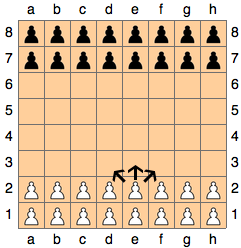
\includegraphics[scale=0.5]{fig1.png}
\caption{Movimento possível da peça e2}
\label{fig:1}
\end{center}
\end{figure}

%Figura 2 (a e b)
\begin{figure}[H]
\begin{center}
\subfloat[Possibilidades para a peça f3]{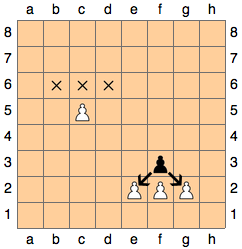
\includegraphics[scale=0.5]{fig2a.png}\label{fig:2a}}\hspace{10px}
\subfloat[Captura de e2]{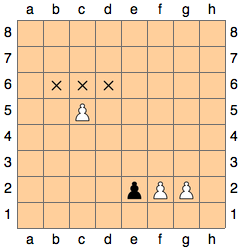
\includegraphics[scale=0.5]{fig2b.png}\label{fig:2b}}
\caption{Processo de captura.}
\label{fig:2}
\end{center}
\end{figure}

\subsection{Vitória}
\begin{enumerate}
\item O primeiro jogador a atingir a base do adversário, vence. No caso anterior, se o jogador 2 (peças pretas) atingisse a linha 1, venceria.
\item Se todas as peças de um jogador forem capturadas, este perde o jogo.
\item Um empate é matemáticamente impossível, e todas as peças têm sempre pelo menos uma jogada na diagonal possível.
\end{enumerate}


%************************************************************************************************
%************************************************************************************************
\newpage

\section{Arquitectura do Sistema}
% Descrever em linhas gerais o sistema e os módulos que o constituem. Deve ser abordada 
% a comunicação com o visualizador, que mesmo que ainda não esteja implementada, já
% deverá estar pensada. Assim, deve ser incluída a sintaxe das mensagens a trocar com o visualizador.

O jogo do Breakthrough foi constitúido tendo em base três módulos elementares. Estados todos eles interligados, seja directa, ou indirectamente, através de um intermediário. Estes módulos estão listados do menos geral para o menos específico, uma vez que consoante aparecem na seguinte lista, o módulo numéricamente acima, consome o módulo numéricamente abaixo.

\begin{enumerate}
\item Módulo de Lógica.
\item Módulo de Interacção.
\item Módulo de Comunicação.
\end{enumerate}



%************************************************************************************************

\subsection{Módulo de Lógica}

Este é módulo mais importante de todo este trabalho, porque é aquele que trata da lógica toda associada ao mesmo, fazendo mover o "motor" do jogo e tratando das
operações mais básicas que definem as regras do mesmo.

É aqui que são definidos os predicados que são utilizados pelos predicados mais gerias para a validação das jogadas, inicialização do tabuleuro, verificação de um vencedor - seja por ter conseguido chegar a linha de partida do adversario, ou por ter adquirido todas as pessas do seu oponente. Também fazem parte deste módulo, os predicados da inteligência artificial do módo Humano/Computador.


%************************************************************************************************

\subsection{Módulo de Interacção}

Este módulo, consome o \textit{Módulo de Lógica}, e serve de interface para o utilizador e/ou para o módulo de comunicação.

Aqui sao definidos os predicados que facilitam a interacção com o jogo, e dada a sua generalidade, podem ser utilizadas pra diferentes fins, como anteriormente referido.

\begin{code}[H]
	\begin{verbatimtab} % verbatimtab para codigo com tabs


initDynBoard(+Side, -Board).
isWinner(+Board, +/-Player).
checkMove(+Board, +Ox, +Oy, +Dx, +Dy, +Player).
movePawn(+Board, +Ox, +Oy, +Dx, +Dy, -NewBoard).
pickNextMove(+Board, +Side, +Player, -Ox, -Oy, -Dx, -Dy).
\end{verbatimtab}
\caption{Fazem parte deste módulo predicados tais como:}
\end{code}

%************************************************************************************************

\subsection{Módulo de Comunicação}

Este é módulo que serve como servidor do jogo, que possibilita a comunicação com qualquer programa externo e possibilta por sua vez a
comunicação com um visualisador a ser implementado posteriormente.
Este módulo consome os serviços que o \textit{Módulo de Interacção} tem para oferecer, e disponibliza-os de uma forma ainda mais geral que anteriormente, possibilitando
assim uma vasta utilização do motor do jogo, bem como a sua difusão para meios diferentes e externos ao mesmo.

\begin{code}[H]
	\begin{verbatimtab} % verbatimtab para codigo com tabs


...
\end{verbatimtab}
\caption{Fazem parte deste módulo predicados tais como:}
\end{code}


%************************************************************************************************
%************************************************************************************************
\newpage

\section{Módulo de Lógica do Jogo}
% Descrever o projecto e implementação do módulo Prolog, incluindo a forma de
% representação do estado do tabuleiro,  verificação do cumprimento das regras do
% jogo, determinação do final do jogo e cálculo das jogadas a realizar pelo computador
% utilizando diversos níveis de jogo.



%************************************************************************************************

\subsection{Representação do Estado do Jogo}
% \textit{estado(?Tabuleiro).}

A representação do tabuleiro é feita em Prolog por uma lista de listas.
O tabuleiro é quadrado - número de linhas igual ao número de colunas - e dinâmico, podendo assumir valores compreendidos entre 5 e 19, inclusivé.

Cada item do tabuleiro é representado no formato ``Jogador", em que este pode ser:
\begin{itemize}
\item 1 - jogador de peças brancas (Norte)
\item 2 - jogador de peças pretas (Sul)
\item 0 - casa vazia
\end{itemize}

\begin{code}[H]
	\begin{verbatimtab}
initDynBoard(Side, Board)
\end{verbatimtab}
\caption{Inicializa tabuleiro dinâmico}
\end{code}

Este predicado inicializa o tabuleiro \textit{Board} com nº de linhas/colunas \textit{Side}.

\begin{code}[H]
	\begin{verbatimtab}
B = [
	[1,1,1,1,1],
	[1,1,1,1,1],
	[0,0,0,0,0],
	[2,2,2,2,2],
	[2,2,2,2,2]
	]
\end{verbatimtab}
\caption{Ex. de chamada a \textit{initDynBoard(5, B)}}
\end{code}

%************************************************************************************************

\subsection{Visualização do Estado do Jogo}

\textit{printBoard(+Tabuleiro).}

Esta função apresenta as células do tabuleiro representadas pelo número do jogador correspondente, ou em branco, caso a mesma se encontre vazia.
Apresenta também as linhas e colunas à volta do tabuleiro, numeradas do número 1 até ao número da ordem de colunas ou linhas.
\begin{code}[H]
	\begin{verbatimtab}
initDynBoard(8, Board),
printBoard(Board).
\end{verbatimtab}
\caption{Predicado para gerar e imprimir um tabuleiro de 8x8}
\end{code}

% Figura do tabuleiro
\begin{figure}[h!]
\begin{center}
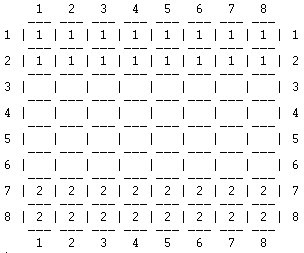
\includegraphics[scale=1]{fig_tab.png}
\caption{Tabuleiro impresso com ``printBoard', mostrando o estado inicial de um jogo'.}
\label{fig:3}
\end{center}
\end{figure}

\newpage

%************************************************************************************************

\subsection{Validação de Jogadas}
 \textit{checkCorrectPlayer(+Jogador, +Peão)}

Predicado que valida a escolha de um peão.

Se o jogador \textit{X} escolher um peão correspondente ao jogador \textit{Y} ou a uma casa vazia, é exibido o erro \textit{"Casa inválida, tente novamente"}, e o predicado retorna \textit{False}.

\textit{ checkMove(+Tabuleiro, +Origem x, +Origem y, +Destino x, +Destino y, +Jogador) }

Predicado que valida uma jogada, de acordo com as regras de jogo descritas na secção 2.2 .

%************************************************************************************************

\subsection{Execução de Jogadas}
% \textit{executa\_movimento(+Jogada, + Tabuleiro, -NovoTabuleiro).}

\textit{movePawn(+Tabuleiro entrada, +Origem x, +Origem y, +Destino x, +Destino y, +Tabuleiro saída)}

Este predicado encapsula \textit{checkMove()} e \textit{getPawn()}.
Se a jogada for válida, o valor da casa (\textit{Destino x}, \textit{Destino y)} é substituido pelo
peão que se encontra na casa (\textit{Origem x}, \textit{Origem y}) e devolvido em \textit{NovoTabuleiro}.

\textit{getPawn(+Tabuleiro, +X, +Y, -Valor)}

Predicado usado para retornar o valor da casa (X,Y) - 0, 1 ou 2.

%************************************************************************************************

\subsection{Lista de Jogadas Válidas}
% \textit{lista\_jogadas(+Tabuleiro, -ListaJogadas).}



%************************************************************************************************

\subsection{Avaliação do Tabuleiro}
% \textit{avalia\_tabuleiro(+Tabuleiro, -Valor).}



%************************************************************************************************

\subsection{Final do Jogo}
% \textit{fim\_jogo(+Tabuleiro, -Vencedor).}



%************************************************************************************************

\subsection{Cálculo da Jogada do Computador}
% \textit{calcula\_jogada(+Nível, +Tabuleiro, -Jogada).}



%************************************************************************************************

\subsection{Recepção de mensagem do visualizador}
% \textit{recebe\_mensagem(+ Mensagem, - Resposta).}



%************************************************************************************************
%************************************************************************************************
\newpage

\section{Conclusões e Perspectivas de Desenvolvimento}

% Que conclui da análise do jogo e da pesquisa bibliográfica realizada?
% Como vai ser desenvolvido o trabalho?
% Que parte (\%) do trabalho estima que falta fazer?

Dados os conhecimentos adquiridos, podemos concluir que o código dos predicados para efetuar quer um movimento, quer uma captura, deverá ser simples de implementar. 
O trabalho já começou a ser desenvolvido em Prolog, e posteriormente será criado um interface em ambiente gráfico no contexto de LAIG.

Por enquanto, a implementação incidirá apenas no ambiente em modo de texto.

Estimamos que cerca de 15\% do total do projeto esteja concluído, uma vez que os modos de jogo Humano/Computador e Computador/Computador, sendo baseadas na implementação de algoritmos de inteligência artificial, irão necessitar de mais investigação, e por conseguinte mais tempo dispendido.

Olhando otimisticamente para o projeto, achamos que a sua relativa simplicidade nos permitirá desenvolver a lógica de jogo suficientemente depressa para nos podermos concentrar em pequenos detalhes que tornarão o jogo o mais interessante possível.


%************************************************************************************************
%************************************************************************************************

\clearpage

\addcontentsline{toc}{section}{Bibliografia}
\renewcommand\refname{Bibliografia}
\bibliographystyle{plain}
\bibliography{myrefs}

\nocite{breakSite}
\nocite{tut1}
\nocite{tut2}


%************************************************************************************************
%************************************************************************************************
\newpage

\appendix
\section{Código Prolog}

\lstset{ %
language=Prolog,                % choose the language of the code
basicstyle=\footnotesize,       % the size of the fonts that are used for the code
numbers=left,                   % where to put the line-numbers
numberstyle=\footnotesize,      % the size of the fonts that are used for the line-numbers
stepnumber=1,                   % the step between two line-numbers. If it is 1 each line will be numbered
numbersep=5pt,                  % how far the line-numbers are from the code
backgroundcolor=\color{white},  % choose the background color. You must add \usepackage{color}
commentstyle=\color{blue},
showspaces=false,               % show spaces adding particular underscores
showstringspaces=false,         % underline spaces within strings
showtabs=false,                 % show tabs within strings adding particular underscores
frame=single,   		% adds a frame around the code
tabsize=2,  		% sets default tabsize to 2 spaces
captionpos=b,   		% sets the caption-position to bottom
breaklines=true,    	% sets automatic line breaking
breakatwhitespace=false,    % sets if automatic breaks should only happen at whitespace
escapeinside={\$}{)},          % if you want to add a comment within your code
caption={Descriptive Caption Text}
}


\lstset{literate=%
{á}{{\'a}}1
{Á}{{\'A}}1
{é}{{\'e}}1
{É}{{\'E}}1
{í}{{\'i}}1
{Í}{{\'I}}1
{ó}{{\'o}}1
{Ó}{{\'O}}1
{ú}{{\'u}}1
{Ú}{{\'U}}1
{ç}{{\c{c}}}1
{Ç}{{\c{C}}}1
{ã}{{a}}1
{Ã}{{A}}1
{à}{{\`a}}1
{À}{{\`A}}1
}

\begin{lstlisting}


% ****************************************************************
% Inicialização do servidor.
% ****************************************************************


:-use_module(library(sockets)).

port(60001).

server:-
		port(Port),
		socket_server_open(Port,Socket),
		write('Breakthrough server started on port ['), write(Port), write(']'), nl,
		write('Waiting for connection...'), nl,
		socket_server_accept(Socket, _Client, Stream, [type(text)]),
		write('Connection received'), nl,
		server_loop(Stream),
		socket_server_close(Socket),
		write('Server Exit'),nl.

server_loop(Stream) :-
		repeat,
			read(Stream, ClientRequest),
			write('Received: '), write(ClientRequest), nl, 
			server_input(ClientRequest, ServerReply),
			format(Stream, '~q.~n', [ServerReply]),
			write('Send: '), write(ServerReply), nl, 
			flush_output(Stream),
		(ClientRequest == bye; ClientRequest == end_of_file), !.

% Initialize board
server_input(initialize(Side), ok(Board)):- 
		initDynBoard(Side, Board), !.

% Execute Move	
server_input(execute(Board, Ox-Oy, Dx-Dy), ok(NewBoard)):- 
		movePawn(Board, Ox, Oy, Dx, Dy, NewBoard), !.

% Calculate next Move
server_input(calculate(Board, Player), ok(Ox-Oy, Dx-Dy, NewBoard)):- 
		length(Board, Side),
		pickNextMove(Board, Side, Player, Ox, Oy, Dx, Dy ),
		movePawn(Board, Ox, Oy, Dx, Dy, NewBoard), !.
	
% Check Winner
server_input(game_end(Board), ok(Winner)):- 
		isWinner(Board, Winner), !.
	
	
server_input(bye, ok):-!.
server_input(end_of_file, ok):-!.
server_input(_, invalid) :- !.



% ****************************************************************
% ****************************************************************
% Jogo
% ****************************************************************
% ****************************************************************

:-use_module(library(random)).


% ****************************************************************
% ****************************************************************

% Imprime a peça do jogador correspondente.
writePlayer(1) :-
		write(1).
writePlayer(2) :-
		write('2').
writePlayer(0) :-
		write(' ').


% ****************************************************************
% Imprime o número da coluna ou da linha, com um espaço à esqueda
% ou à direita, de forma ao tabuleiro ser disposto correctamente
% com linhas ou colounas de número superior a 9.
% printSpaceNumberL(+N)
% printSpaceNumberR(+N)
% ****************************************************************

printSpaceNumberL(N) :-
		N < 10,
		write(N), write(' ').
		
printSpaceNumberL(N) :-
		write(N).
                
printSpaceNumberR(N) :-
		N < 10,
		write(' '), write(N).

printSpaceNumberR(N) :-
		write(N).

% ****************************************************************
% printRow(+[H|T])
% ****************************************************************

% Critério de paragem.
% Imprime também a borda direita da última célula de cada linha.
printRow([]).

% Imprime a borda esquerda da célula, e a respectivo
% peça do jogador (cabeça da lista).
% Por fim chama recursivamente a mesma função com
% a cauda da lista, até encontrar o critério de paragem.
printRow([H|T]) :-
		write('| '),
		writePlayer(H),
		write(' '),
		printRow(T).


% ****************************************************************
% ****************************************************************

% Imprime a linha de separação horizontal.
printHorizSepp(S,S) :- !.

printHorizSepp(S, N) :-
		N1 is N+1,
		printHorizSepp(S, N1),
		write('--- ').


printHorizSep(S)   :-
		write('    '),
		printHorizSepp(S, 0).

% Imprime os números das colunas.
%printColNumbers([], _).

printColNumbers([_], N) :-
		printSpaceNumberR(N),
		!.

printColNumbers([_|T], N) :-
		N1 is N+1,
		printSpaceNumberR(N),
		write('  '),
		printColNumbers(T, N1).

printColNumbers([H|T]) :-
		write('    '),
		printColNumbers([H|T], 1).


% ****************************************************************
% ****************************************************************

% Critério de paragem.
printFullRow([], _, _).


% Imprime o número da linha no ínicio e no fim de cada iteração,
% bem como o separador horizontal. Chama também o predicado que irá
% imprimir todas as células de cada linha, com a respectiva peça.
% Por fim chama recursivamente a mesma função com a cauda da
% lista (contendo as restantes células da linha correspondente),
% e o número actual da linha, até atingir o critério de paragem,
% ou seja, quando a a cauda for uma lista vazia.
printFullRow([H|T], N, S) :-
		N1 is N+1,
		printHorizSep(S),
		nl,
		printSpaceNumberR(N),
		write(' '),
		printRow(H),
		write('| '),
		printSpaceNumberL(N),
		nl,
		printFullRow(T, N1, S).


% ****************************************************************
% ****************************************************************

% Regra a ser usada quando é passado um tabuleiro vazio.
printBoard([]).

% Imprime o tabuleiro, chamando o predicado que imprime o número
% das colunas (no início e no fim do tabuleiro),
% e de seguida o predicado que imprime cada linha individual.
% É imprimido também o separador horizontal do tabuleiro.
printBoard([H|T]) :-
		length([H|T], S),
		printColNumbers([H|T]),
		nl,
		printFullRow([H|T], 1, S),
		printHorizSep(S),
		nl,
		printColNumbers([H|T]).


% ****************************************************************
% getPawn(+Tabuleiro, +X, +Y, -Jogador)
% Retorna o número do jogador na posição (X,Y) do Tabuleiro.
% Recorre a getPawnPos() para percorrer o tabuleiro.
% ****************************************************************

% Condição de paragem, encontrou a casa.
% Retorna InTabH
getPawnPos([Player|_], Dest, Dest, Player) :- !.

% Percorre o tabuleiro
getPawnPos([_|InTabT], Dest, BaseIncrement, Value) :-
		Increment is BaseIncrement + 1,
		getPawnPos(InTabT, Dest, Increment, Value).

% Verifica se X e Y estão dentro dos valores permitidos
% Recorre a getPawnPos para percorrer o tabuleiro e encontra o jogador
getPawn(InTab, X, Y, Player) :-
		X > 0,
		Y > 0,
		length(InTab, Len),
		X =< Len,
		Y =< Len,
		getPawnPos(InTab, Y, 1, L),
		getPawnPos(L, X, 1, Player).

        
% ****************************************************************
% getll(Linha,Coluna,Tabuleiro,Valor)
% Obter o valor da casa
% ****************************************************************

% Obtem o valor de determinada posição N numa Lista.
getl(Lista,N,Valor) :-
		getl(Lista,N,1,Valor).

getl([H|_],N,N,H) :- !.

getl([_|R],N,Nactual,Valor) :-
		NR is Nactual+1,
		getl(R,N,NR,Valor).

% ****************************************************************
% Obtem o valor de determinada posição (Linha,Coluna) num Tabuleiro
% ****************************************************************
getll(Linha,Coluna,Tabuleiro,Valor) :-
		% Obtemos primeiro uma Linha completa
		getl(Tabuleiro,Linha,Lista),
		% Obtemos o valor da coluna na Linha obtida
		getl(Lista,Coluna,Valor).

                 
                 
% ****************************************************************
% substll(Tabuleiro,Linha, Coluna, Valor, Resultado)
% Substitui a peça de uma Casa por outra
% ****************************************************************

substl(Lista,N,Valor,Resultado) :-
        substl(Lista,N,1,Valor,[],Resultado).

substl([],_,_,_,NovaLista,NovaLista).

substl([_|R],N,N,Valor,NovaLista,Resultado) :- !,
		append(NovaLista,[Valor],NovaNovaLista),
		NR is N+1,
		substl(R,N,NR,Valor,NovaNovaLista,Resultado).

substl([H|R],N,Nactual,Valor,NovaLista,Resultado) :-
		append(NovaLista,[H],NovaNovaLista),
		NR is Nactual+1,
		substl(R,N,NR,Valor,NovaNovaLista,Resultado).

substll(Tabuleiro,Linha, Coluna, Valor, Resultado) :-
		getl(Tabuleiro,Linha,Lista),
		substl(Lista,Coluna,Valor,NovaLista),
		substl(Tabuleiro,Linha,NovaLista,Resultado).

% ****************************************************************
% Verificação de um vencedor
% ****************************************************************

checkForInvasion([]).
checkForInvasionOfP1([]).

% Verificar se há peças do jogador 1 na última linha
% (Último predicado a ser executado)
checkForInvasionOfP1([InTabT], Player) :-
		member(1, InTabT),
		Player is 1,
		!.

% Corrre resto do tabuleiro recursivamente.
checkForInvasionOfP1([_|InTabT], Player) :-
		checkForInvasionOfP1(InTabT, Player).

% Verificar se há peças do jogador 2 na primeira linha
% (Primeiro predicado a ser executado).
checkForInvasion([InTabH|_], Player) :-
		member(2, InTabH),
		Player is 2,
		!.

% Se não encontrar peças do jogador 2, corre
% recursivamente o resto do tabuleiro até chegar à ultima linha.
checkForInvasion([_|InTabT], Player) :-
		checkForInvasionOfP1(InTabT, Player).

% Verifica se existe pelo menos 1 peça do jogador P
hasPieces([], _).
hasPieces([H|T], P) :-
		\+(member(P, H)),
		hasPieces(T, P).


% Predicado principal
% O jogador é vencedor se 1 de 2 casos acontecer:
% 1. tiver chegado à base adversária
% 2. o adversário não tiver peças.
isWinner(Tab, 1) :-
		checkForInvasion(Tab, 1);
		hasPieces(Tab, 2).

isWinner(Tab, 2) :-
		checkForInvasion(Tab, 2);
		hasPieces(Tab, 1).

% ****************************************************************
% Validação de uma jogada
% ****************************************************************

% checkMove(+Tab, +Ox, +Oy, +Dx, +Dy, +P)
% Valida movimentos exclusivamente verticais

% JOGADOR 1
% Movimento vertical
checkMove(Tab, Ox, Oy, Ox, Dy, 1) :-
		!,
		Dy =:= Oy+1,
		getPawn(Tab, Ox, Dy, P),
		P = 0.

% Movimento diagonal
checkMove(Tab, Ox, Oy, Dx, Dy, 1) :-
        Dy =:= Oy+1,
		Dx =:= Ox+1,
		getPawn(Tab, Dx, Dy, P),
		P \= 1.

checkMove(Tab, Ox, Oy, Dx, Dy, 1) :-
        Dy =:= Oy+1,
		Dx =:= Ox-1,
		getPawn(Tab, Dx, Dy, P),
		P \= 1.

% JOGADOR 2
% Movimento vertical
checkMove(Tab, Ox, Oy, Ox, Dy, 2) :-
		!,
		Dy =:= Oy-1,
		getPawn(Tab, Ox, Dy, P),
		P = 0.

% Movimento diagonal
checkMove(Tab, Ox, Oy, Dx, Dy, 2) :-
		Dy =:= Oy-1,
		Dx =:= Ox+1,
		getPawn(Tab, Dx, Dy, P),
		P \= 2.

checkMove(Tab, Ox, Oy, Dx, Dy, 2) :-
		Dy =:= Oy-1,
		Dx =:= Ox-1,
		getPawn(Tab, Dx, Dy, P),
		P \= 2.


% ****************************************************************
% Move player
% ****************************************************************

switchPlayer(1,2).
switchPlayer(2,1).

movePawn(Tab, Ox, Oy, Dx, Dy, TabOut) :-
		getPawn(Tab, Ox, Oy, Me),
		checkMove(Tab, Ox, Oy, Dx, Dy, Me),
		getPawn(Tab, Dx, Dy, Opponent),
		Opponent = 0,
		substll(Tab, Dy, Dx, Me, TabTmpOut),
		substll(TabTmpOut, Oy, Ox, 0, TabOut).

movePawn(Tab, Ox, Oy, Dx, Dy, TabOut) :-
		getPawn(Tab, Ox, Oy, Me),
		checkMove(Tab, Ox, Oy, Dx, Dy, Me),
		getPawn(Tab, Dx, Dy, Opponent),
		Opponent \= 0,
		substll(Tab, Dy, Dx, Me, TabTmpOut),
		substll(TabTmpOut, Oy, Ox, 0, TabOut).

%movePawn(Tab, _, _, _, _, Tab).




% ****************************************************************
% Inicializa dinamicamente do o tabuleiro
% initDynBoard(+Side, -Board)
% ****************************************************************

initDynBoard_line(BaseNumber, BaseNumber, _, Line, Line).

initDynBoard_line(BaseNumber, Side, V, LineIn, LineOut) :-
		N is BaseNumber + 1,
		initDynBoard_line(N, Side, V, [V|LineIn], LineOut).
		
                
initDynBoard_col(BaseNumber, BaseNumber, Board, Board).

initDynBoard_col(BaseNumber, Side, BoardIn, BoardOut) :-
		L is BaseNumber + 1,
		(
				( L =:= 1 ; L =:= 2 ) ->
						X is 2 ;
						( ( L =:= Side ; L =:= Side - 1 ) ->
								X is 1 ;
								X is 0
						)
		),
		initDynBoard_line( 0, Side, X, [], Y ),
		initDynBoard_col(L, Side, [Y|BoardIn], BoardOut).

initDynBoard(Side, Board) :-
		Side > 4,
		Side < 20,
		initDynBoard_col(0, Side, [], Board).
        
        
% ****************************************************************
% ****************************************************************      

checkPoss_prior(X, X, _, _, _, _, 0):- !.
checkPoss_prior(_, _, 1, _, 2, 0, 3):- !.
checkPoss_prior(_, _, 1, _, 2, 1, 4):- !.
checkPoss_prior(_, _, S, S, 1, 0, 3):- !.
checkPoss_prior(_, _, S, S, 1, 2, 4):- !.
checkPoss_prior(_, _, _, _, 1, 2, 2):- !.
checkPoss_prior(_, _, _, _, 2, 1, 2):- !.
checkPoss_prior(_, _, _, _, _, 0, 1):- !.
checkPoss_prior(_, _, _, _, _, _, 0):- !.


checkPoss(Board, Side, Player, Ox, Dx, Dy, ListIn, ListOut) :-
		Dx > 0,
		Dx =< Side,
		Dy > 0,
		Dy =< Side,
		getPawn(Board, Dx, Dy, Pawn),
		checkPoss_prior(Ox, Dx, Dy, Side, Player, Pawn, Prior),
		append( ListIn, [Prior], ListOut ).
		
checkPoss(_, _, _, _, _, _, ListIn, ListOut) :-
		append( ListIn, [0], ListOut ).
		

% ****************************************************************
% ****************************************************************   
		
getPossiblePlays_int(Board, Side, Player, Ox, Dy, Plays) :-
		Dx1 is Ox-1,
		Dx2 is Ox+1,
		checkPoss(Board, Side, Player, Ox, Dx1, Dy, [], Lista1),
		checkPoss(Board, Side, Player, Ox, Ox , Dy, Lista1, Lista2),
		checkPoss(Board, Side, Player, Ox, Dx2, Dy, Lista2, Plays).

		
		
% getPossiblePlays/7		

getPossiblePlays(Board, Side, 1, Ox, Oy, Dy, Plays) :-
		Dy is Oy + 1,
		getPossiblePlays_int(Board, Side, 1, Ox, Dy, Plays).
		
getPossiblePlays(Board, Side, 2, Ox, Oy, Dy, Plays) :-
		Dy is Oy - 1,
		getPossiblePlays_int(Board, Side, 2, Ox, Dy, Plays).
		
getPossiblePlays(_, _, _, _, _, _, [0, 0, 0]).
		

% getPossiblePlays/5
getPossiblePlays(Board, Side, X, Y, Plays) :-
		getPawn(Board, X, Y, Pawn),
		getPossiblePlays(Board, Side, Pawn, X, Y, _, Plays).
		

% ****************************************************************
% ****************************************************************

getMoves([], _, _, _, _, Moves, Moves).

getMoves([P|Tail], Inc,  Ox,Oy, Dy,  MovesIn, MovesOut) :-
		P > 0,
		Inc2 is Inc + 1,
		NewX is Ox + Inc - 1,
		getMoves(Tail, Inc2, Ox,Oy, Dy, [P-Ox-Oy-NewX-Dy|MovesIn], MovesOut).			

getMoves([_|Tail], Inc, Ox,Oy, Dy, MovesIn, MovesOut) :-
		Inc2 is Inc + 1,
		getMoves(Tail, Inc2, Ox,Oy, Dy, MovesIn, MovesOut).
		
		
% ****************************************************************
% ****************************************************************
	
addMoves(Board, Side, Player, Player, X, Y, MovesIn, MovesOut) :-
		getPossiblePlays(Board, Side, Player, X, Y, Y2, Plays),
		getMoves(Plays, 0, X, Y, Y2, MovesIn, MovesOut).

addMoves(_, _, _, _, _, _, Moves, Moves).		


% ****************************************************************
% ****************************************************************

checkNextMoves_line([], _, _, _, _, _, Moves, Moves).
checkNextMoves_line([Cell|LineTail], Board, Side, X, Y, Player, MovesIn, MovesOut) :-
		X1 is X + 1,
		addMoves(Board, Side, Cell, Player, X, Y, MovesIn, MovesOutTemp),
		checkNextMoves_line(LineTail, Board, Side, X1, Y, Player, MovesOutTemp, MovesOut).
	

% checkNextMoves/7
checkNextMoves([], _, _, _, _, Moves, Moves).
checkNextMoves([Line|BoardTail], Board, Side, Y, Player, MovesIn, MovesOut) :-
		Y1 is Y + 1,
		checkNextMoves_line(Line, Board, Side, 1, Y, Player, MovesIn, MovesOutTemp),
		checkNextMoves(BoardTail, Board, Side, Y1, Player, MovesOutTemp, MovesOut).

% checkNextMoves/4
checkNextMoves(Board, Side, Player, MovesOut) :-
		checkNextMoves(Board, Board, Side, 1, Player, [], MovesOut).


% ****************************************************************
% ****************************************************************

% getMaxPriority/3

getMaxPriority([], Priority, Priority).

getMaxPriority([Prior-_-_-_-_|Tail], PriorIn, PriorOut) :-
		Prior > PriorIn,
		getMaxPriority(Tail, Prior, PriorOut).

getMaxPriority([_|Tail], PriorIn, PriorOut) :-
		getMaxPriority(Tail, PriorIn, PriorOut).

		
% getMaxPriority/2
getMaxPriority(List, Priority) :-
		getMaxPriority(List, 0, Priority).
		

% ****************************************************************
% ****************************************************************

% buildMaxPriorityList/6

buildMaxPriorityList([], _, Total, Total, List, List).

buildMaxPriorityList([Pri-Ox-Oy-Dx-Dy|MovesTail], Priority, TotalIn, TotalOut, ListIn, ListOut) :-
		Pri = Priority,
		TotalIn2 is TotalIn + 1,
		buildMaxPriorityList(MovesTail, Priority, TotalIn2, TotalOut, [Ox-Oy-Dx-Dy|ListIn], ListOut).

buildMaxPriorityList([_|MovesTail], Priority, TotalIn, TotalOut, ListIn, ListOut) :-
		buildMaxPriorityList(MovesTail, Priority, TotalIn, TotalOut, ListIn, ListOut).

% buildMaxPriorityList/4
buildMaxPriorityList(Moves, Priority, Total, ListOut) :-
		buildMaxPriorityList(Moves, Priority, 0, Total, [], ListOut).


% ****************************************************************
% ****************************************************************

% getMoveNumber/7

getMoveNumber([Ox-Oy-Dx-Dy|_], PickNumber, PickNumber, Ox, Oy, Dx, Dy).

getMoveNumber([_|MovesTail], N, PickNumber, Ox, Oy, Dx, Dy) :-
		N < PickNumber,
		N2 is N + 1,
		getMoveNumber(MovesTail, N2, PickNumber, Ox, Oy, Dx, Dy).

% getMoveNumber/6
getMoveNumber(List, PickNumber, Ox, Oy, Dx, Dy) :-
		getMoveNumber(List, 0, PickNumber, Ox, Oy, Dx, Dy).


% ****************************************************************
% ****************************************************************

pickNextMove(Board, Side, Player, Ox, Oy, Dx, Dy ) :-
		checkNextMoves(Board, Side, Player, Moves),
		getMaxPriority(Moves, Priority),
		buildMaxPriorityList(Moves, Priority, Total, List),
		random(0, Total, Random),
		getMoveNumber(List, Random, Ox, Oy, Dx, Dy).
		
		
% ****************************************************************
% ****************************************************************

checkAbort('sair') :-
		abort.
checkAbort('Sair') :-
		abort.
checkAbort('SAIR') :-
		abort.
checkAbort(_).

readIntegerAbort(Text, Value) :-
		write(Text),
		read(Input),
		checkAbort(Input),
		integer(Input),
		Value = Input.
		
readXY(X,Y) :-
		readIntegerAbort('X = ', X),
		readIntegerAbort('Y = ', Y).
		
printPlayer(Player) :-
		nl, nl,
		write('[Jogador: '),
		write(Player),
		write(']'), nl.

checkCorrectPlayer(Player, 0) :- !,
		write('Casa inválida, tente novamente!'), nl,
		Pawn \= 0.
		
checkCorrectPlayer(Player, Pawn) :-
		Player \= Pawn,
		!,
		write('Esse peão não é seu, tente novamente!'), nl,
		Player = Pawn.
		
checkCorrectPlayer(Pawn, Pawn).

% ****************************************************************
% ****************************************************************

verificaVencedor(Board, _, _, _) :-
		isWinner(Board, Player),
		nl,nl,
		write('Jogo terminado! Jogador ['),
		write(Player),
		write('] venceu o jogo'), nl.
	
verificaVencedor(Board, Side, GameMode, Player) :-
		printPlayer(Player),
		play(Board, Side, GameMode, Player).
	
% ****************************************************************
% ****************************************************************

transitPlay(BoardIn, Side, GameMode, Player, Ox, Oy, Dx, Dy) :-
		movePawn(BoardIn, Ox, Oy, Dx, Dy, Board),
		write('Jogador ['), write(Player), write('] moveu a peça ['),
		write(Ox), write(','), write(Oy), write('] para ['),
		write(Dx), write(','), write(Dy), write(']'), nl, nl,
		printBoard(Board),
		switchPlayer(Player, NextPlayer),
		verificaVencedor(Board, Side, GameMode,NextPlayer).

transitPlay(Board, Side, GameMode, 1, _, _, _, _) :- !,
		write('Jogada Inválida, tente outra vez!'), nl,
		play(Board, Side, GameMode, 1).


% ****************************************************************
% ****************************************************************

play(Board, Side, 2, 2) :- !,
		pickNextMove(Board, Side, 2, Ox, Oy, Dx, Dy ),
		transitPlay(Board, Side, 2, 2, Ox, Oy, Dx, Dy ).

play(Board, Side, GameMode, Player) :- !,
		repeat,
		nl,
		write('Peça a mover?'), nl,
		readXY( Ox, Oy ), nl,
		getPawn(Board, Ox, Oy, Pawn),
		checkCorrectPlayer(Player, Pawn),
		repeat,
		write('Casa de destino?'), nl,	
		readXY( Dx, Dy ), nl,
		transitPlay(Board, Side, GameMode, Player, Ox, Oy, Dx, Dy ).
	
play(Board, Side, GameMode) :-
		play(Board, Side, GameMode, 1).


% ****************************************************************
% ****************************************************************
	
init :-
		repeat,
		readIntegerAbort('Lado do tabuleiro [5,19] = ', Side), nl,
		Side >= 5,
		Side =< 19,
		initDynBoard(Side, Board),
		repeat,
		write('Modo de jogo:'), nl,
		write('1 - Humano/Humano'), nl,
		write('2 - Humano/Computador'), nl,
		readIntegerAbort('> ', Mode), nl,
		Mode > 0,
		Mode < 3,
		printBoard(Board),
		printPlayer(1),
		play(Board, Side, Mode).


\end{lstlisting}


\end{document}
